\documentclass{report}
\usepackage[utf8]{inputenc}
\usepackage{url}
\usepackage{graphicx}
\graphicspath{ {images/} }
\usepackage[nottoc]{tocbibind}
\usepackage[toc, page]{appendix}
\setlength{\parindent}{4em}
\setlength{\parskip}{1em}

\title{Audit of SSH Client - PuTTY}
\author{Alok Vaidya\\[1cm]{\large Supervisor: Dr. David Oswald}}
\date{August 14, 2017}

\begin{document}

\maketitle
\tableofcontents
\chapter{Preamble}
\section{Abstract}
The Secure Shell (SSH) protocol provides a mechanism to securely run network services over an insecure network. It is most commonly used for remote logins to shell accounts on Unix/Linux or other computer systems. PuTTY is an SSH client program running commonly on a Windows system providing users a means to connect securely to a remote server. We performed a security audit of PuTTY with the purpose of finding vulnerabilities that, if exploited, would allow an attacker to compromise the security of an SSH connection. We primarily focused our attention on the Diffie-Hellman (DH) Key Exchange that leads to the establishment of a shared key that is used to encrypt all subsequent communication and on the Public Key Authentication mechanism used to authenticate the user to the server. We also analyzed randomness generation process, modular exponentiation implementations and supported legacy protocols. We performed a code review of the software in order to find possible vectors for known attacks and conclude that implementations of cryptographic primitives within the software employ all necessary safeguards to nullify such vectors.
\section{Keywords}
SSH, PuTTY, Diffie-Hellman, Timing Attacks
\chapter{Introduction}
\section{Overview}
In this chapter we provide a summary of the entire project to the audience. It begins by outlining the Secure Shell (SSH) protocol and the PuTTY Software. We move forward by detailing the workings of Key Exchange and Public Key Authentication within the SSH protocol. It lists the goals and objectives we set out to achieve with this project. Lastly it explains the setup of the environment for the analysis we perform mentioning some of the tools we use.

\section{SSH and PuTTY}
SSH is a cryptographic network protocol used to provide secure network services over an unsecured network
\footnote{\url{https://en.wikipedia.org/wiki/Secure_Shell}}
The most common use of SSH is to remotely login to computer systems securely. Users on their computers use SSH clients that connect to an SSH server running on the server (remote) machine. PuTTY\footnote{\url{https://www.chiark.greenend.org.uk/~sgtatham/putty/}} is an SSH client software that runs most commonly on Windows systems. The PuTTY project among other programs includes Plink - a command-line interface to the PuTTY back ends and PuTTYgen - a RSA and DSA key generation utility. In the next section we introduce the workings of PuTTY with emphasis on the DH Key Exchange and the Public Key Authentication sections.
\section{Diffie-Hellman Key Exchange}
To establish a session the SSH client initiates the connection to the SSH server and announces its own name and version along with the SSH version it implements. The server responds with a similar message identifying itself and its SSH version. Both the client and server must now establish a shared key that will be used to encrypt the message traffic for this session. This method to establish one-time session keys is known as Key Exchange. SSH clients and servers support multiple algorithms for Key Exchange \cite{rfc4253} such as DH, Elliptic Curve DH, RSA etc. For the specific purpose of this section we will assume that the client and the server have agreed upon the DH Group Exchange protocol.\par

Fig. 2.1 provides an overview of the DH Key Exchange process. Once the client and server have agreed upon the DH group parameters, the server sends the client suitable \textit{g} (generator for the DH group) and a corresponding prime \textit{p}. The client generates a secret exponent \textit{a} and computes \(e\ = \ g^a\ mod\ p\) and sends it to the server.The server computes a random exponent of its own, say \(b\) and sends \(f\ =\ g^b\ mod\ p\) to the client. In DH, \(a\) is known as Alice's (client's) secret and \(b\) as Bob's (server's) secret. On receiving \(e\) the server computes \(K\ =\ e^b\ mod\ p\)  i.e. \(g^{ab} \ mod\ p\) similarly the client computes \(K\ =\ f^b\ mod\ p\) i.e. \(g^{ba}\ mod\ p\). It's critical that both of the secret exponents \(a\) and \(b\) remain secret from an attacker. If either are somehow revealed, the attacker can compute the shared secret \(K\) by himself as both \(e\) and \(f\) are sent in plain text across the network. Once the client and the server both share a secret key, all subsequent communication is encrypted using the shared secret.
\begin{figure}[ht]
\caption{Exchange of messages during DH Key Exchange}
\centering
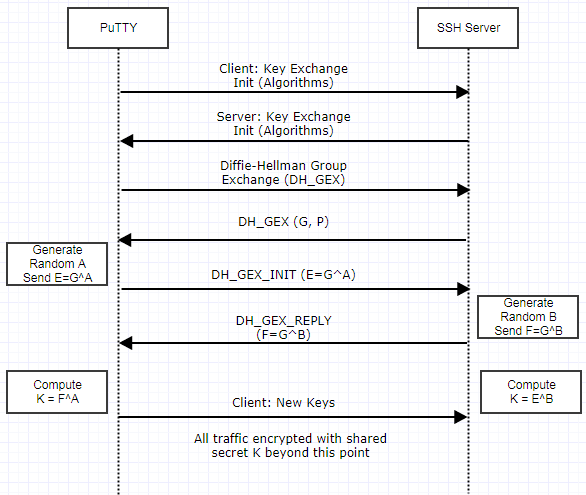
\includegraphics[width=1\textwidth]{SSH_DH_KEX.png}
\end{figure}
\section{Public Key Authentication}
A SSH server authenticates a user using either a password or a public key mechanism. When using public key authentication, the possession of a private key serves as authentication \cite{rfc4252}. The SSH client creates a signature using the user's private key. The server check whether public key is a valid authentication mechanism for the user and that the signature verifies. If both the conditions hold the access is granted. Fig. 2.2 offers an overview of the process\par
\begin{figure}[ht]
\caption{Exchange of messages during Public Key Authentication}
\centering
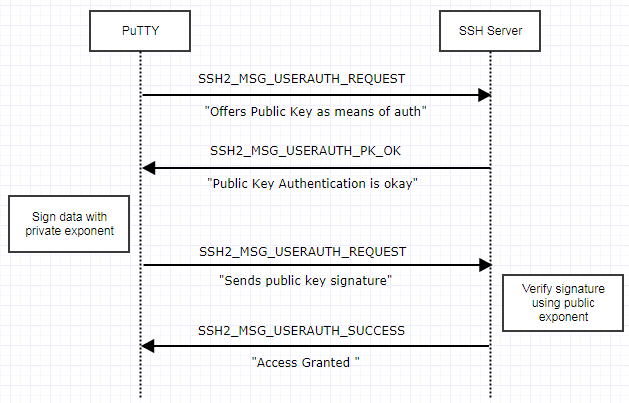
\includegraphics[width=1\textwidth]{SSH_PK_Auth.png}
\end{figure}
\section{Objectives}
\par
Now that we have briefly described the DH Key Exchange and the Public Key Authentication processes of SSH, we move onto outlining the key objectives of the project.\par
As specified earlier our primary objective is to find timing leaks in implementations cryptographic primitives and in that regard we look closely at both the DH Key Exchange and Public Key Authentication portions of the source code. Within this implementations the sections of particular interest to us is the modular exponentiation operations. Both, the DH Key Exchange - during the computation of \(g^a\ mod\ p\) - and the Public Key Authentication - while creating the signature - use modular exponentiation. Both these processes use cryptographically sensitive data in their respective modular exponentiations and a timing leak in these operations could leak the sensitive data. Analysis of these processes is described in chapters 4 and 5.\par

Cryptographic primitives often require a random number generator that generates a random stream of bits. To ensure safety of sensitive data it is critical that this stream of bits be strictly random. To this end our next objective is to analyze and review the code responsible for randomness (a.k.a noise) generation. Additionally to test the statistical properties of the random numbers, we subject them to a variety of test suits. Randomness generation analysis is described in chapter 6\par
In line with our goal of a security audit of the entire software our next objective concerns performing an exhaustive analysis of all invocations of the modular exponentiation operation. This analysis aims to confirm that the data passed to each invocation is safe from tampering by an attacker. By manipulating data to such invocations information about sensitive data could be possibly leaked. Chapter 7 comprises of this analysis.\par
Lastly we analyze and review the implementation of some of the legacy protocols that PuTTY supports. Chapter 8 provides the details of this analysis.\par
\section{Environment Setup}
This section is supposed to acquaint the reader with the setup used for testing and measurements. We describe the audit process and methodology in the next chapter.\par

The source code of PuTTY was downloaded from the PuTTY homepage \cite{putty} and compiled on Windows 7 OS using Microsoft Visual Studio 2015. The source code provides solutions for all PuTTY projects including those mentioned in section "SSH and PuTTY". Compiling a solution for a project rendered an executable for the corresponding project. For debugging and flow control analysis the solution for PuTTY was used in the debug mode. This allowed to set breakpoints and variable watch on necessary sections of code. For automated measurements a Plink executable was created with required additions to the code for logging data values and time measurements. This executable was then called from a Java program iteratively. Check Appendix "A: Automated Mesaurements" for details. For both debugging and automated measurements a Bitvise SSH Server running on the same host was used as the server. Alternatively for simulating messages across a network an OpenSSH server running on a Raspberry Pi machine was used.
"Appendix B: Software and Tools" lists all software and tools used along with the version details.
\chapter{Methodology}
\chapter{Diffie-Hellman Key Exchange Analysis}
\chapter{Public Key Authentication Analysis}
\chapter{Randomness Generation Analysis}
\chapter{Modular Exponentiation Analysis}
\chapter{Legacy Protocols Analysis}
\chapter{Conclusions}
\chapter{Further Work}
\section{Overview}
This chapter provides overview of work that can be undertaken as an extension of this project. Carrying out tasks listed here shall make for a broader security audit of the software and weren't included in this project due to time restrictions.
\section{Cache-based Timing Attacks}
\section{Buffer Overflows}
\begin{appendices}
\chapter{Automated Measurements}
\chapter{Software and Tools}
\end{appendices}
\begin{thebibliography}{9}
\bibitem{putty}
PuTTY
\url{https://www.chiark.greenend.org.uk/~sgtatham/putty/}
\bibitem{rfc4251}
RFC 4251, The Secure Shell (SSH) Protocol Architecture,\\
\url{https://tools.ietf.org/html/rfc4251}
\bibitem{rfc4252}
RFC 4252, The Secure Shell (SSH) Authentication Protocol,\\  \url{https://tools.ietf.org/html/rfc4252}
\bibitem{rfc4253}
RFC 4253, The Secure Shell (SSH) Transport Layer Protocol,\\ \url{https://tools.ietf.org/html/rfc4253}
\bibitem{rfc4254}
RFC 4254, The Secure Shell (SSH) Connection Protocol,\\ \url{https://tools.ietf.org/html/rfc4254}
\bibitem{randeval}
Randomness Evaluation Framework of Cryptographic Algorithms,\\
\url{http://www.academia.edu/9902264/Randomness_Evaluation_Framework_of_Cryptographic_Algorithms}
\end{thebibliography}
\listoffigures
\end{document}
